% Stage 3 report, revision 2 (reviewer comments applied): recap of the steady model, transient
% calibration, the transient predictor, validation on generated floorplans, robustness, the tool.
% Compile from this folder: pdflatex stage3_v2.tex (twice).
\documentclass[11pt,a4paper]{article}
\usepackage[margin=2.2cm]{geometry}
\usepackage[T1]{fontenc}
\usepackage{lmodern}
\usepackage{amsmath}
\usepackage{graphicx}
\usepackage{booktabs}
\usepackage{array}
\usepackage{enumitem}
\usepackage{xcolor}
\usepackage{caption}
\usepackage{float}
\usepackage[section]{placeins}
\usepackage[hidelinks]{hyperref}
\graphicspath{{../../experiments/}}
\setlist{itemsep=1pt,topsep=3pt}
\setlength{\parindent}{0pt}
\setlength{\parskip}{4pt}
\captionsetup{font=small,labelfont=bf}
\newcommand{\us}{\,$\mu$s}
\newcommand{\degC}{\,\textdegree C}

\begin{document}

\begin{center}
{\LARGE\bfseries Lightweight Temperature Predictor:}\\[4pt]
{\Large\bfseries TapaSense}\\[8pt]
{\large Stage 3 Report: Transient Predictor, Robustness and Validation}\\[6pt]
Ethan Bobby Kurien \quad Kaivalya Mase
\end{center}

%=====================================================================
\section{Recap: the steady-state model (Stage 2)}\label{sec:recap}
This report is about transient prediction. This section collects what it builds on from Stage 2.

\textbf{Floorplans.} The main set is 24 floorplans: the 23 given ones and HET-A, our own
heterogeneous layout. Each has $N = 8$ cores (2 big, 6 little). Some experiments use the
\emph{main subset}, one floorplan per style: s1\_fp001, s2\_fp004, s3\_fp002 and s4\_fp001.

\textbf{HotSpot is linear.} Without leakage, doubling every power doubles every temperature rise
above ambient, and the rise caused by several cores together is the sum of the rises each causes
alone (checked to $10^{-6}$\,K). So a 1\,W test in each core is enough to describe the chip.

\textbf{S1, the influence matrix.} The steady temperature of every block is
\begin{equation}
  T = T_\text{amb} + G\,P,
  \label{eq:s1}
\end{equation}
where $P$ is the vector of core powers (W), $T_\text{amb}$ the ambient temperature, and $G$ the
\emph{influence matrix}: $G_{ij}$ is the steady temperature rise of block $i$ (K) per watt in core
$j$. Column $j$ of $G$ is measured directly by one steady HotSpot run with 1\,W in core $j$, so
8 runs (about 4\,s) calibrate a floorplan.
\begin{itemize}
  \item \textbf{Exact.} S1 reproduces HotSpot to its 6-decimal output (0.00003\,K worst on 7{,}248
        test runs) and always picks the right hottest core.
  \item \textbf{Cheap.} One matrix--vector product per prediction (2.6\us) and 928\,B per
        floorplan (464\,B in 32-bit numbers).
  \item \textbf{Calibration is needed.} Every calibration-free alternative (a generic heat-spread
        kernel, or $G$ borrowed from another floorplan or predicted from geometry) was 0.5--2.7\,K
        off on average and up to 12\,K.
\end{itemize}
\textbf{S1-hot-max.} A core's average hides its hottest point, which is 3--9\,K hotter. Each of
the 8 calibration runs also gives HotSpot's full $64\times64$ temperature map, so the same
Equation~\eqref{eq:s1} can be written for every grid cell. S1-hot-max predicts all cells of each
core and takes the maximum. It is exact; stored in full it needs 115\,kB, and about 3\,kB after
dropping the cells that can never be the hottest.

\textbf{On the 52 generated floorplans} of Section~\ref{sec:gen}, S1 was off by
$6.5\times10^{-6}$\,K on average and $3.4\times10^{-5}$\,K at worst (the same as on the main set),
and picked the right hottest core on every floorplan.

%=====================================================================
\section{Transient calibration}
Because HotSpot is linear, its temperature response to any power trace is fixed by the response
to a 1\,W step in each core. Transient calibration therefore records these step responses, and the
transient model is a compact fit to them.

\subsection{Planned step runs}
For each of the 24 floorplans, in addition to the 8 steady runs:
\begin{itemize}
  \item \textbf{8 short step runs:} 1\,W switched on in one core at $t = 0$, temperatures sampled
        every 1\,ms for 2\,s (the fast part of the response).
  \item \textbf{8 long step runs:} the same step, sampled every 20\,ms for 100\,s (the slow heat
        sink).
  \item \textbf{Merging:} the short run is used up to 2\,s and the long run after it, giving one
        step response $s_{ij}(t)$ per pair of cores from 1\,ms to 100\,s.
  \item \textbf{Cost:} all 24 runs take about 5 CPU-minutes per floorplan. The 24 floorplans took
        66\,min of \emph{wall time} (real elapsed time on the clock) with 8 HotSpot runs going
        \emph{in parallel} (8 runs at the same time, each on its own processor core).
\end{itemize}

\textbf{What $s_{ij}(t)$ is.} $s_{ij}(t)$ is the temperature rise of core $i$ at time $t$ after
1\,W is switched on in core $j$. It is the transient version of the influence-matrix entry: it
starts at 0 and, once the chip settles, ends at $G_{ij}$, so $s_{ij}(\infty) = G_{ij}$.

The responses span very different speeds: time constants of about 1\,ms, 3\,ms, 26\,ms, 89\,ms,
0.56\,s and 8.1\,s (a time constant $\tau$ is how long a part of the chip takes to cover about
two-thirds of its rise). About 70\,\% of a core's self-heating appears within 10\,ms.

\textbf{T1, one time constant (baseline).} The simplest transient model lets each block move a
fixed fraction of the way towards its S1 steady value at every time step:
\begin{equation}
  x_i[k+1] = a_i\, x_i[k] + (1 - a_i)\,(G\,P[k])_i, \qquad a_i = e^{-\Delta t/\tau_i},
  \qquad T_i = T_\text{amb} + x_i,
  \label{eq:t1}
\end{equation}
where $x_i$ is block $i$'s rise above ambient, $\Delta t$ the time step (1\,ms), and $\tau_i$ one
time constant per block, fitted so that its step response $G_{ij}(1 - e^{-t/\tau_i})$ is as close
as possible to the measured $s_{ij}(t)$.

\textbf{T3, sum of exponentials.} Each step response is written as a sum of $M$ rising curves:
\begin{equation}
  s_{ij}(t) \approx \sum_{m=1}^{M} a_{ijm}\left(1 - e^{-t/\tau_m}\right),
  \qquad \sum_m a_{ijm} = G_{ij}.
  \label{eq:t3}
\end{equation}
\begin{itemize}
  \item \textbf{The curves $1 - e^{-t/\tau_m}$ are the same for every pair of cores.} The $M$ time
        constants $\tau_1, \dots, \tau_M$ belong to the chip and package (silicon, spreader, sink),
        not to a particular pair.
  \item \textbf{Only the weights $a_{ijm}$ differ between pairs.} They say how much of the
        $i \leftarrow j$ heating happens at each speed.
  \item \textbf{The weights of each pair add up to $G_{ij}$}, so T3 ends at exactly S1's value:
        it is exact in steady state.
\end{itemize}
\textbf{Fitting.} If the time constants were known, the best weights would follow from ordinary
linear least squares (a straight line fit, in many dimensions). So the fit has two layers: an inner
layer solves the weights exactly for a guess of the $\tau_m$, and an outer search (SciPy's
\texttt{least\_squares}) adjusts the $\tau_m$ until the leftover error stops shrinking. This
two-layer method is known as variable projection~\cite{golub73}.

\textbf{Running T3.} At run time, T3 keeps one number $z_{jm}$ per core $j$ and time constant $m$
($N \times M$ numbers) and updates them every time step $k$:
\begin{equation}
  z_{jm}[k+1] = \lambda_m z_{jm}[k] + (1-\lambda_m) P_j[k],\qquad \lambda_m = e^{-\Delta t/\tau_m},
  \qquad x_i[k+1] = \sum_{j,m} a_{ijm} z_{jm}[k+1].
  \label{eq:t3run}
\end{equation}
\begin{itemize}
  \item $P_j[k]$: power of core $j$ (W) during step $k$, taken as constant within the step.
  \item $\Delta t$: the time step (1\,ms). $\tau_m$: the $m$-th time constant (s).
  \item $\lambda_m$: the fraction of $z_{jm}$ kept from one step to the next, between 0 and 1;
        close to 1 for slow time constants.
  \item $z_{jm}$ (W): a running average of core $j$'s power that forgets old values at speed
        $\tau_m$. This is what \emph{filter} means here: a fast filter follows the power almost
        immediately, a slow one (the heat sink) only after seconds. It starts at 0 (cold chip).
  \item $x_i$: the rise of block $i$ above ambient (K), so $T_i = T_\text{amb} + x_i$.
\end{itemize}
For power that is constant during each step, Equation~\eqref{eq:t3run} reproduces the fitted step
responses exactly at every step. Sums of exponentials of this kind are the standard way to compute
transients of compact thermal models~\cite{pagani15}.

\begin{center}
\small
\begin{tabular}{@{}l c c@{}}
\toprule
Model & Worst fit error (24 floorplans) & Size \\
\midrule
T1 (one time constant per block) & 14.1\,K & 1.0\,kB \\
T3, $M=2$ & 2.82\,K & 1.9\,kB \\
T3, $M=3$ & 1.04\,K & 2.8\,kB \\
T3, $M=4$ & 0.46\,K & 3.7\,kB \\
T3, $M=6$ & 0.12\,K & 5.6\,kB \\
\bottomrule
\end{tabular}
\end{center}
One time constant (T1) cannot follow a response spanning 1\,ms to 8\,s. T3 converges quickly with
$M$.

\begin{figure}[H]
  \centering
  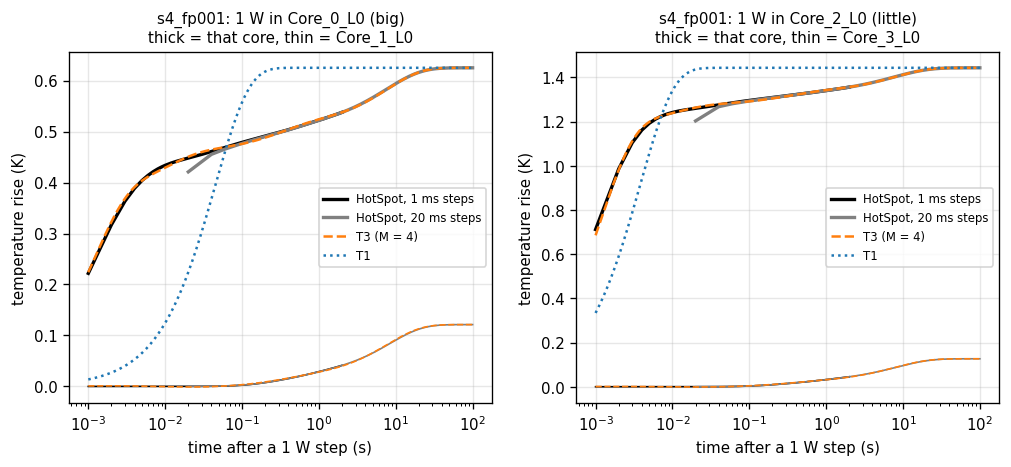
\includegraphics[width=0.9\linewidth]{P1-1_step_calibration/results/step_response_fits.png}
  \caption{Step responses to 1\,W in a big core (left) and a little core (right), log time axis.
  HotSpot (black and grey) and T3 (orange dashed) overlap; T1 (blue dotted) has the right final
  value but the wrong shape. Thin lines: coupling to a neighbouring core. The responses keep rising
  until about 30--100\,s: this is the heat sink.}
\end{figure}

\subsection{Calibration from one long trace (ARX)}\label{sec:arx}
Instead of planned steps, we recorded one long HotSpot trace and fitted ARX models (T2,
``AutoRegressive with eXogenous input''), the classic system-identification model also used for
temperature prediction in~\cite{coskun09,singla15}.

\textbf{Calibration trace.} 60\,s at 1\,ms steps on each main-subset floorplan, from a cold chip.
Every core switches independently between random power levels, with phases of 1\,ms to 5\,s, so
both fast and slow behaviour is excited. The first 1, 5, 20 or 60\,s were used for fitting.

\textbf{The model.} The next temperature rise above ambient is a weighted mix of the last few rises
and powers. With $n_a$ past rises and $n_b$ powers, written ARX$(n_a, n_b)$:
\begin{equation}
  x[k] = \sum_{l=1}^{n_a} A_l\, x[k-l] + \sum_{l=0}^{n_b-1} B_l\, P[k-l].
  \label{eq:arx}
\end{equation}
For example, ARX(2,2) is
\[
  x[k] = A_1 x[k-1] + A_2 x[k-2] + B_0 P[k] + B_1 P[k-1].
\]
Here $x$ is the vector of rises, of every block (``all blocks'') or of the 8 cores only (``cores only'', which is what on-chip
sensors measure); $A_l$ and $B_l$ are matrices of coefficients.

\textbf{Fitting.} Every step of the trace gives one equation~\eqref{eq:arx} in the unknown
coefficients (1{,}000 equations per second of trace); all of them are solved together by linear
least squares.

\textbf{Steady gain constrained to $G$.} If the power stays constant, ARX settles at
\[
  x = \Big(I - \sum_l A_l\Big)^{-1} \sum_l B_l\, P.
\]
We force this to equal S1's $G\,P$ by computing $B_0$
from that rule instead of fitting it, so ARX is exact in steady state, like T3. Nothing in the fit,
however, forces ARX to be \emph{stable}.

\begin{center}
\small
\begin{tabular}{@{}l c c c c@{}}
\toprule
Model (mean / worst) & 1\,s trace & 5\,s & 20\,s & 60\,s \\
\midrule
ARX (2,2), all blocks & 9.5 / 79\,K & 0.31 / 1.2\,K & 0.21 / 1.03\,K & 0.32 / 1.3\,K \\
ARX (3,3), all blocks & 5.2 / 67\,K & unstable & unstable & unstable \\
ARX (3,3), cores only & 4.6 / 51\,K & 0.40 / 1.5\,K & 0.32 / 0.95\,K & 0.39 / 0.96\,K \\
T3 $M=4$ from step runs & \multicolumn{4}{c}{0.062 / 0.31\,K} \\
\bottomrule
\end{tabular}
\captionof{table}{ARX against T3 on the main subset. Columns: length of the recorded trace used to
fit ARX. Each entry is the mean / worst absolute error over the 8 cores on two unseen 10\,s test
traces per floorplan, run open loop from a cold chip (the model sees only the power, never
HotSpot's temperatures). ``Unstable'': the prediction grew without bound.}
\label{tab:arx}
\end{center}

\begin{itemize}
  \item \textbf{A trace must be at least about 5\,s long}, or the slow heat sink is never seen. Our
        own evidence: the slowest fitted time constant is 8.1\,s, the step responses in Figure~1
        keep rising until about 30--100\,s, and a 1\,s trace gives 5--10\,K mean error. This
        matches the usual picture of a packaged chip, where the heat spreader and sink are by far
        the slowest part of the thermal path~\cite{skadron03,hotspot}.
  \item \textbf{Beyond about 20\,s the error rises again.} Least squares minimises the error of one
        step ahead, which is already tiny and the same for every trace length, while the test runs
        the model on its own outputs for 10{,}000 steps. The slow heat sink appears in ARX as a
        \emph{pole} very close to 1: a factor by which the remaining slow part of the rise is
        multiplied at every step (about 0.9999 here, like $\lambda_m$ in
        Equation~\eqref{eq:t3run}). A change in the fourth decimal of such a factor is invisible
        over one step but adds up to tenths of a kelvin over 10{,}000 steps.
  \item \textbf{Too many lags can make ARX unstable:} with three lags on all blocks the prediction
        blew up on every trace length from 5\,s on (Table~\ref{tab:arx}).
  \item \textbf{T3 from planned steps is 3--5$\times$ more accurate} on the same test traces
        (0.062 / 0.31\,K against at best 0.21 / 0.95\,K) and stable by construction.
\end{itemize}

%=====================================================================
\section{Transient predictor}

\subsection{Following HotSpot over time}
Tested from a cold chip on 2\,s traces on all 24 floorplans, 10\,s traces on the four main-subset
floorplans (s1\_fp001, s2\_fp004, s3\_fp002, s4\_fp001), and a real workload (HotSpot's EV6
floorplan with a gcc power trace).

\begin{center}
\small
\begin{tabular}{@{}l c c c c@{}}
\toprule
Model & Mean error & Worst error & Time per step & Size \\
\midrule
T1 & 7.25\,K & 14.6\,K & 1.5\us & 1.0\,kB \\
T3, $M=2$ & 0.92\,K & 2.9\,K & 3.0\us & 1.9\,kB \\
T3, $M=3$ & 0.19\,K & 1.1\,K & 3.0\us & 2.8\,kB \\
T3, $M=4$ & 0.090\,K & 0.30\,K & 3.1\us & 3.7\,kB \\
T3, $M=6$ & 0.0093\,K & 0.13\,K & 3.2\us & 5.6\,kB \\
T2 ARX (main subset) & 0.19\,K & 0.57\,K & 5.4\us & 6.2\,kB \\
T3 $M=4$ on EV6 + gcc & 0.073\,K & 0.21\,K & 4.4\us & 28.8\,kB \\
\bottomrule
\end{tabular}
\end{center}
Increasing $M$ improves accuracy at the cost of model size; no speed-up or slow-down is observed.

\subsection{Forecasting from sensor readings}
For DTM, the controller knows the current sensor readings and its planned power, and wants the
temperature some steps ahead. HotSpot's core temperatures stand in for the sensors. At 352 points
in each 10\,s test trace (main subset), each model forecasts 1\,ms to 1\,s ahead:
\begin{itemize}
  \item \textbf{Persistence (no model):} ``the temperature will stay what the sensor reads now'',
        $\hat T(k_0 + h) = T_\text{sensor}(k_0)$. Any model must beat this to be worth using.
  \item \textbf{T1 from sensors:} T1 (Equation~\eqref{eq:t1}) started from the measured
        temperatures and run forward on the planned power.
  \item \textbf{T3 open loop:} plain T3 on the power history alone; it never sees a sensor.
  \item \textbf{T3 anchored on sensors:} T3 run on the power history, then shifted by the current
        difference between sensor and model, with the shift held constant over the horizon:
        $\hat T(k_0 + h) = T_3(k_0 + h) + \big(T_\text{sensor}(k_0) - T_3(k_0)\big)$.
        Unlike plain T3, it corrects its own error at the moment of the forecast, so short-range
        forecasts are almost exact, while T3 still supplies how the temperature will \emph{change}
        under the planned power.
  \item \textbf{T2 ARX from sensors:} cores-only ARX(2,2) started from the last two measured
        temperatures.
\end{itemize}

\begin{center}
\small
\begin{tabular}{@{}l c c c c@{}}
\toprule
Model (mean error) & 1\,ms ahead & 10\,ms & 100\,ms & 1\,s \\
\midrule
No model (persistence) & 0.013\,K & 0.11\,K & 0.69\,K & 2.7\,K \\
T1 from sensors & 0.88\,K & 3.6\,K & 4.7\,K & 4.2\,K \\
T3 open loop & 0.06\,K & 0.06\,K & 0.06\,K & 0.06\,K \\
T3 anchored on sensors & 0.0009\,K & 0.0044\,K & 0.017\,K & 0.055\,K \\
T2 ARX from sensors & 0.0013\,K & 0.015\,K & 0.10\,K & 0.42\,K \\
\bottomrule
\end{tabular}
\end{center}
Persistence is fine on average but up to 8\,K wrong 10\,ms ahead, when a power change falls inside
that window. T1 from sensors is worse than no model: its single time constant gets the speed of the
change wrong. Anchored T3 is the best forecaster from 10\,ms to 1\,s.

\begin{figure}[H]
  \centering
  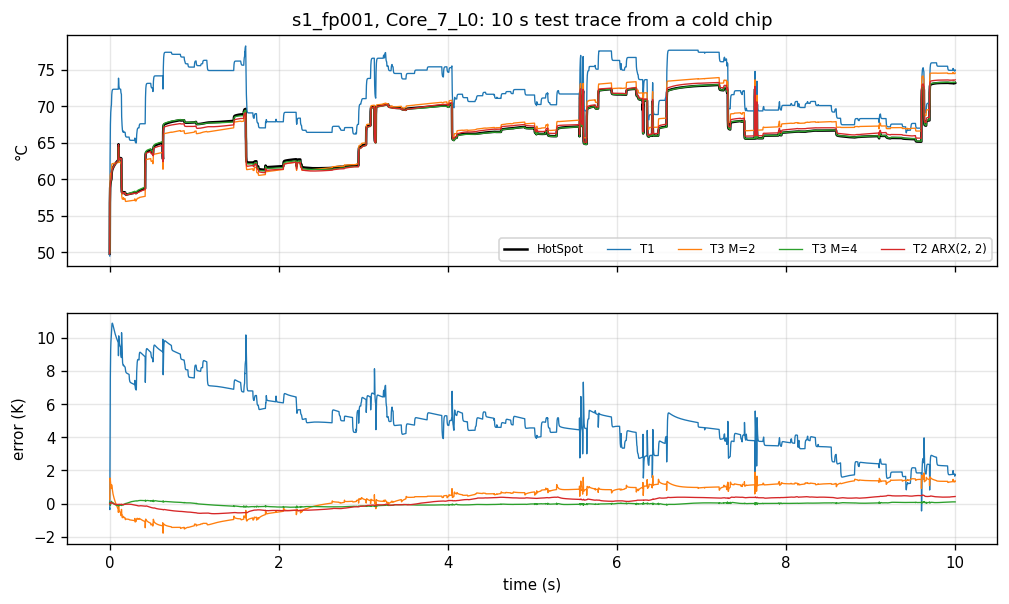
\includegraphics[width=0.48\linewidth]{P3-1_transient_predictor/results/trace_example.png}\hfill
  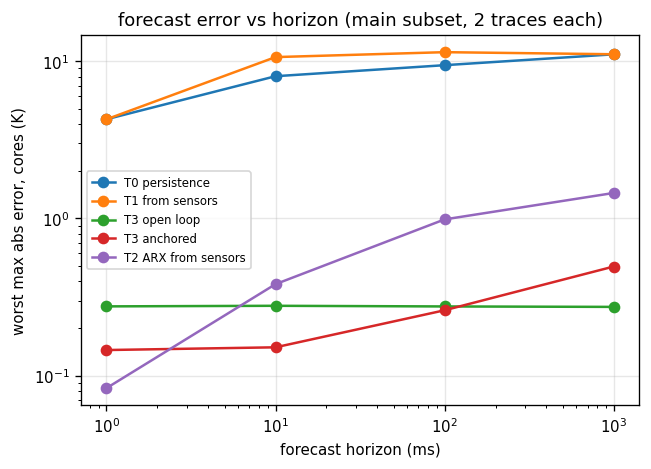
\includegraphics[width=0.48\linewidth]{P3-2_forecast_horizon/results/error_vs_horizon.png}
  \caption{Left: HotSpot and the models on one test trace; T3 sits on top of HotSpot.
  Right: worst forecast error against horizon.}
\end{figure}

\subsection{Trade-offs and the exact model}
Collecting every model's size, worst error and speed in one plot: in the transient case T3 is the
Pareto front from 2 to 6\,kB; each extra time constant costs about 1\,kB and divides the worst
error by 2--4. (In steady state there is no trade-off: S1 is exact.)

As an independent reference (T4), a debug patch makes HotSpot export its internal thermal network
(16{,}396 nodes): $C\,\dot x = -G_\text{net}\,x + B\,P$, with $C$ the heat capacities,
$G_\text{net}$ the thermal conductances and $B$ the map from core powers to nodes. It reproduces
HotSpot to $10^{-6}$\,K and its steady gain equals our calibrated $G$, which confirms S1
independently. Model-order reduction (modal truncation, balanced truncation, and a small filter
for the dropped fast modes) shrinks it to 32 states with 0.047\,K worst error (16\,kB). Without
the fast-mode filter the error stalled at 3.3\,K for every size. Reduced models of this kind are
used for on-chip temperature estimation in~\cite{sharifi08}.

\begin{figure}[H]
  \centering
  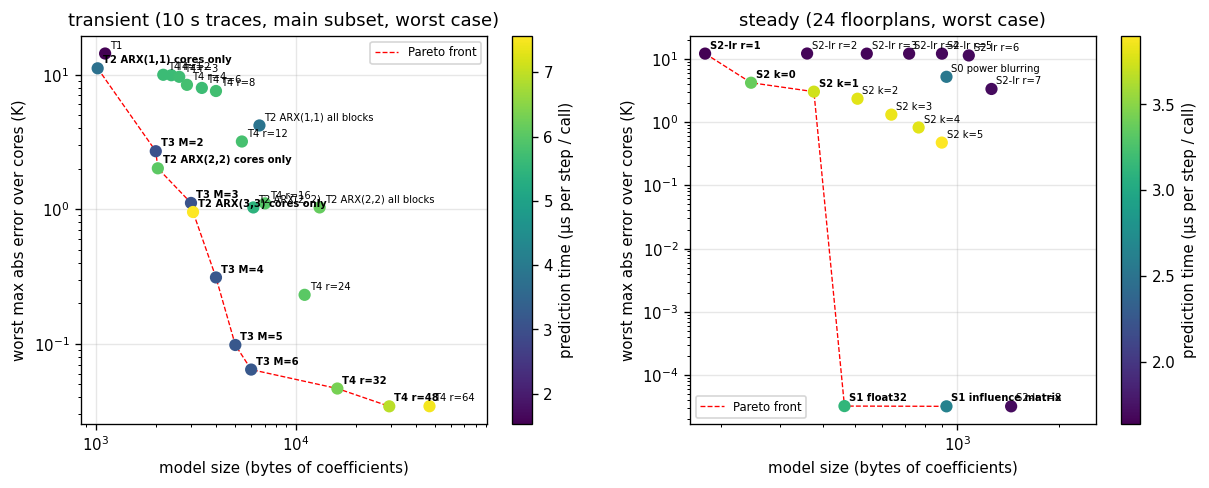
\includegraphics[width=0.48\linewidth]{P3-3_pareto/results/pareto.png}\hfill
  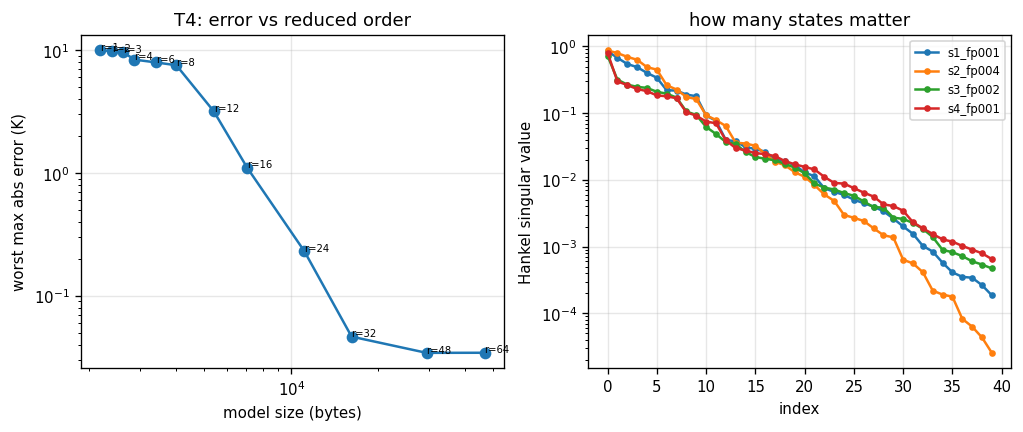
\includegraphics[width=0.48\linewidth]{P3-4_state_space_T4/results/t4_reduction.png}
  \caption{Left: size against worst error for every model; Pareto front in bold.
  Right: T4 error against the number of states.}
\end{figure}

%=====================================================================
\section{The final transient model and its validation on 52 new floorplans}

\subsection{T3 with four time constants}
The transient model is T3 with $M=4$ (Equations~\eqref{eq:t3} and \eqref{eq:t3run}). We compared
four families (T1, T2 ARX, T3, T4) and chose T3 because:
\begin{itemize}
  \item \textbf{It is accurate enough with room to spare:} 0.06--0.09\,K mean and 0.30\,K worst
        error, against targets of 0.5\,K and 1\,K, at 3.1\us\ per step and 3.7\,kB.
  \item \textbf{It is exact in steady state and stable by construction.} The weights of every pair
        sum to $G_{ij}$, so T3 agrees with S1 once power stops changing, and every filter has a
        decay factor $0 < \lambda_m < 1$, so it cannot blow up. ARX is also exact in steady state
        (its gain is constrained to $G$), but nothing guarantees its stability: with three lags it
        blew up (Section~\ref{sec:arx}, Table~\ref{tab:arx}).
  \item \textbf{It is the best accuracy per byte} (the Pareto front from 2 to 6\,kB), and
        $M$ is a single knob: $M=6$ gives 0.13\,K worst for 5.6\,kB if more accuracy is needed.
  \item \textbf{It is the best forecaster for DTM} when anchored on the sensors, from 10\,ms to 1\,s
        ahead.
\end{itemize}
T1 was ruled out because one time constant cannot cover 1\,ms to 8\,s (14\,K worst), and ARX
because it is about 3$\times$ less accurate open loop on the same test traces, needs a long
recorded trace, and can be unstable. T4 is more accurate, but needs HotSpot's internal matrices and
4$\times$ the memory.

\subsection{Testing on 52 generated floorplans}\label{sec:gen}
The models were developed and evaluated on the 24 floorplans of the main set. To check that these
were not a lucky set, we tested them on floorplans they had never seen:
\begin{itemize}
  \item \textbf{Floorplans.} Our generator produced 13 floorplans in each of the four given styles
        (52 in total), with the same cores (2 big, 6 little), the same file format and layer
        stack, and placement rules that imitate each style.
  \item \textbf{Calibration.} Each floorplan was calibrated from scratch exactly as a new user would
        do it: 8 steady runs for S1 and all 24 runs for T3 ($M=4$).
  \item \textbf{Tests.} T3 on a 2\,s phase trace from a cold chip, in which every core switches
        between power levels in phases of 1\,ms to 2\,s (S1 on 302 steady power vectors, see
        Section~\ref{sec:recap}). None of these inputs is used in calibration. Everything ran on
        one laptop in about 100 minutes.
\end{itemize}

\begin{center}
\small
\begin{tabular}{@{}l c c c@{}}
\toprule
Style & Floorplans & T3 mean & T3 worst \\
\midrule
Style 1 & 13 & 0.108\,K & 0.34\,K \\
Style 2 & 13 & 0.114\,K & 0.32\,K \\
Style 3 & 13 & 0.085\,K & 0.31\,K \\
Style 4 & 13 & 0.056\,K & 0.26\,K \\
All generated & 52 & 0.091\,K & 0.34\,K \\
Main set (24 floorplans) & 24 & 0.090\,K & 0.30\,K \\
\bottomrule
\end{tabular}
\end{center}

\begin{figure}[H]
  \centering
  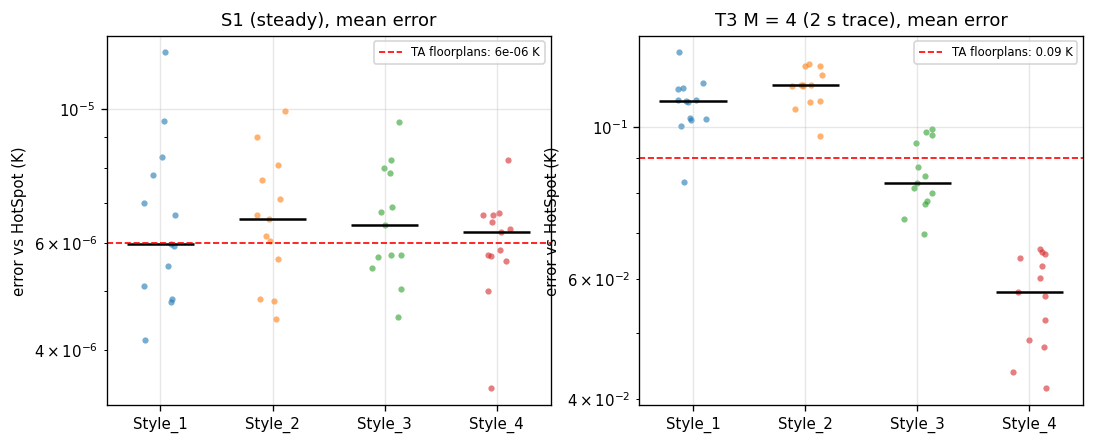
\includegraphics[width=0.48\linewidth]{extended_validation/results/error_by_style.png}\hfill
  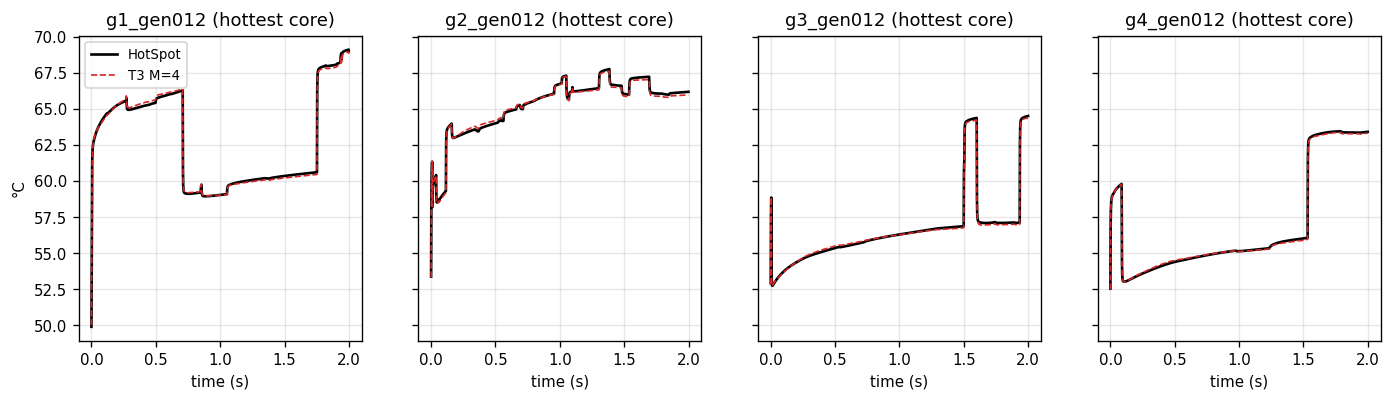
\includegraphics[width=0.48\linewidth]{extended_validation/results/transient_check.png}
  \caption{Left: one dot per generated floorplan, black bar = median, red line = main set.
  Right: the hottest core on a test trace; T3 (red dashed) follows HotSpot (black).}
\end{figure}

\begin{figure}[H]
  \centering
  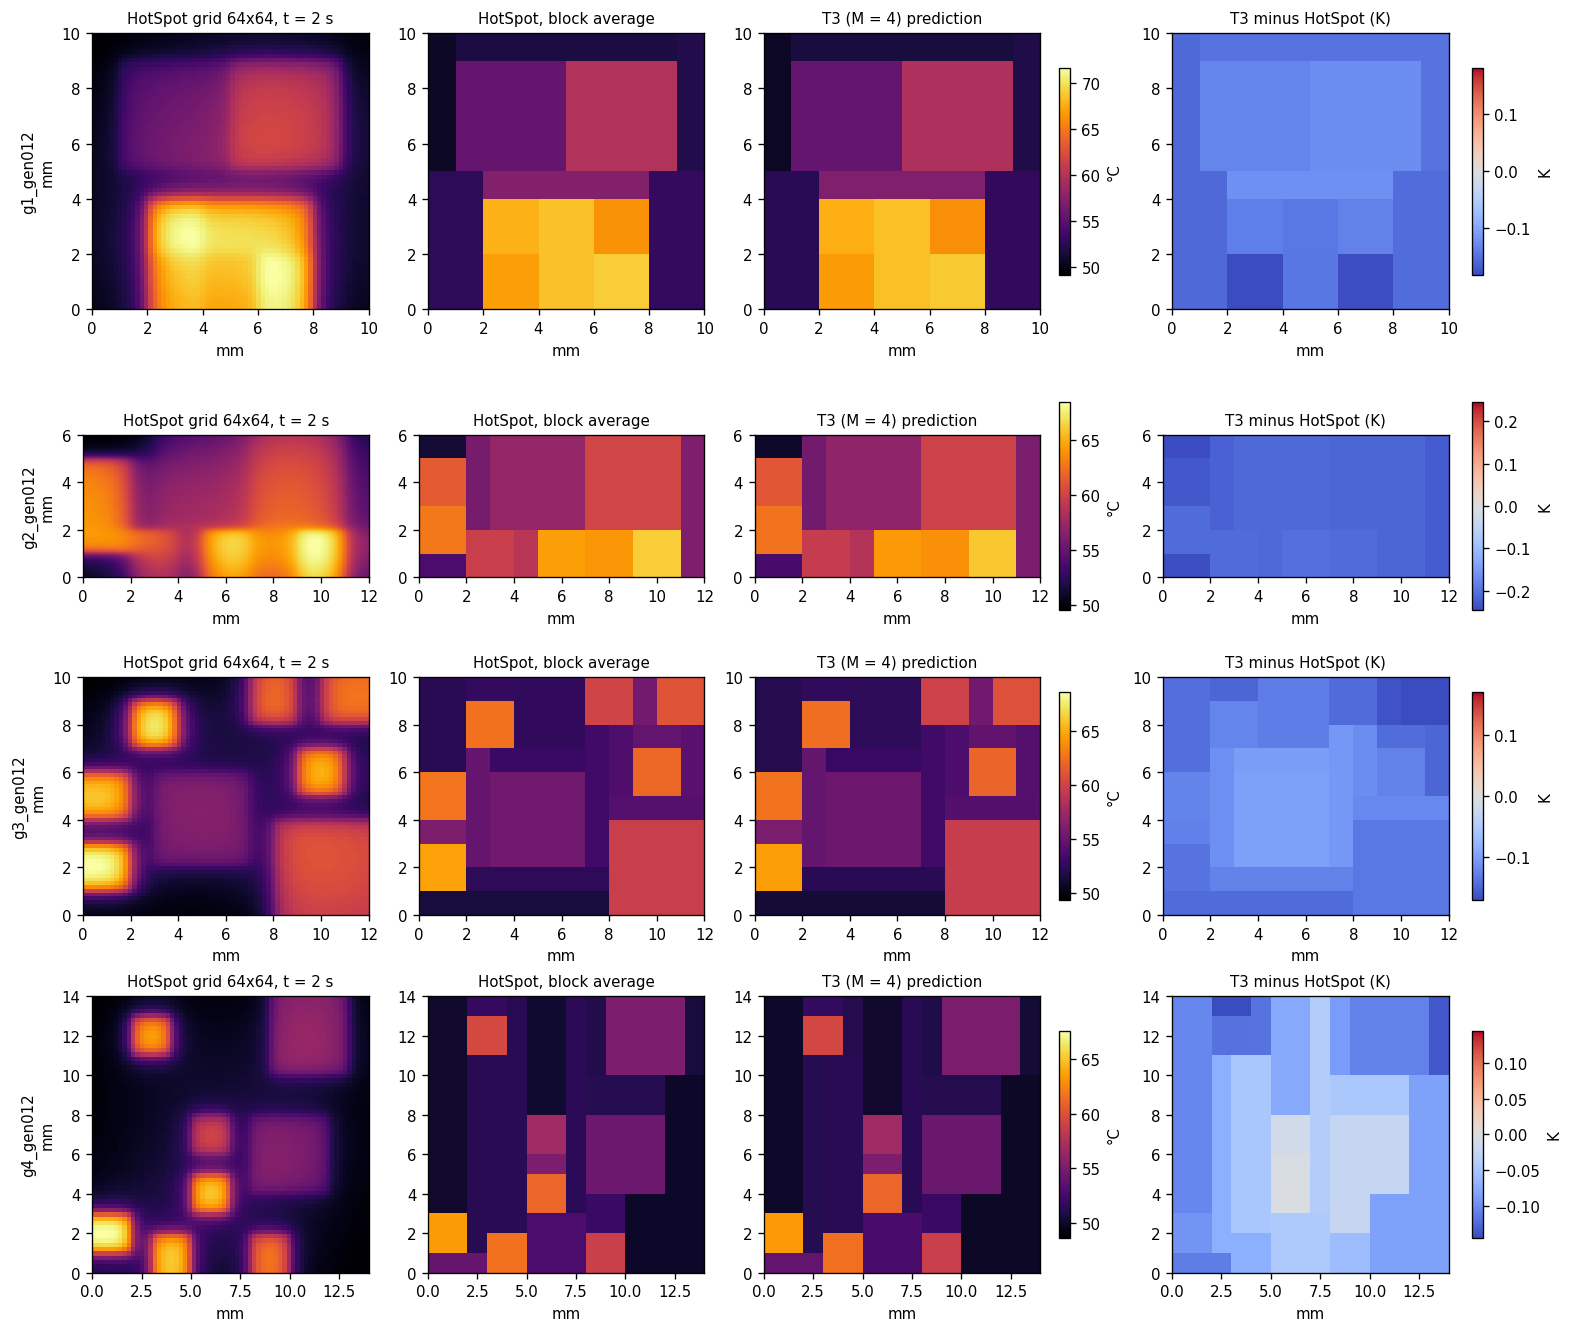
\includegraphics[width=\linewidth]{extended_validation/results/heatmaps_t3.png}
  \caption{T3 at the end of the 2\,s test trace, one generated floorplan per style. Columns:
  HotSpot's $64\times64$ map; HotSpot's block averages; T3's prediction (same colour scale); T3
  minus HotSpot in kelvin.}
\end{figure}

\begin{itemize}
  \item \textbf{The results carry over.} Over 52 new floorplans T3 is off by 0.09\,K on average,
        the same as on the main set. Nothing broke on any floorplan.
  \item \textbf{T3 varies a little with style}, from 0.056\,K (Style 4) to 0.114\,K (Style 2); the
        spread within a style is about as large as between styles. It names the right hottest
        core in 88--100\,\% of steps; misses happen when two cores are within a fraction of a
        kelvin.
  \item \textbf{T3's map matches HotSpot's} within 0.14--0.25\,K in every block at $t = 2$\,s. At
        that moment T3 read slightly cooler than HotSpot in every block (by 0.09--0.21\,K for the
        hottest core). Because T3 can read low, a DTM controller using it should set its
        temperature limit a few tenths of a kelvin below the real limit.
\end{itemize}

%=====================================================================
\section{Robustness}

\subsection{Unusual inputs}
\begin{center}
\small
\begin{tabular}{@{}l c c l@{}}
\toprule
Case (main subset) & T3 mean & T3 worst & Verdict \\
\midrule
Normal trace (reference) & 0.10\,K & 0.32\,K & fine \\
Steady power at 3$\times$ the maximum (S1) & 0.00002\,K & 0.00005\,K & fine \\
Transient at 2$\times$ power & 0.21\,K & 0.64\,K & fine (1\,\% of rise) \\
Bursty power, switching every 1--5\,ms & 0.11\,K & 0.44\,K & fine \\
Task migration between cores & 0.076\,K & 0.31\,K & fine \\
Time step 0.1\,ms instead of 1\,ms & 0.14\,K & 2.16\,K & weak spot \\
Time step 10\,ms & 0.079\,K & 1.88\,K & weak spot \\
Warm start (after the first 50\,ms) & 0.029\,K & 0.27\,K & fine \\
\bottomrule
\end{tabular}
\end{center}
The coefficients are properties of the chip, and hence power levels, bursty power and workload
mapping do not change the relative error (at 2$\times$ power the rise and the error both double;
the error stays about 1\,\% of the rise). A different time step does matter (1--2\,K worst); the
fix is to calibrate at the time step the DTM controller uses.

\subsection{Package changes}
The coefficients belong to one floorplan \emph{and} one package. Setup:
\begin{itemize}
  \item \textbf{Floorplans:} s1\_fp001 and s4\_fp001.
  \item \textbf{Three package changes}, one at a time:
  \begin{itemize}
    \item ambient 35\degC\ instead of 45\degC;
    \item heat-sink convection resistance doubled (0.1 to 0.2\,K/W, a worse cooler);
    \item heat-sink convection resistance halved (0.05\,K/W, a better cooler).
  \end{itemize}
  \item \textbf{Models:} the old models (S1 and T3, $M=4$) and models recalibrated with the usual
        24 runs under the new package.
  \item \textbf{Tests:} 50 random steady power vectors and a 3\,s trace from a cold chip.
\end{itemize}

\begin{center}
\small
\begin{tabular}{@{}l l c c@{}}
\toprule
Change & Model & Steady worst & Transient worst (3\,s) \\
\midrule
Ambient 35\degC & old model, old $T_\text{amb}$ & 10.0\,K & 10.2\,K \\
 & old model, new $T_\text{amb}$ & 0.00001--0.00002\,K & 0.23--0.27\,K \\
 & recalibrated & 0.00001--0.00002\,K & 0.23--0.27\,K \\
\midrule
Convection resistance $\times 2$ & old model & 8.5\,K & 0.43--0.48\,K \\
 & recalibrated & 0.00001--0.00002\,K & 0.26--0.29\,K \\
\midrule
Convection resistance $\times 0.5$ & old model & 4.4\,K & 0.42--0.48\,K \\
 & recalibrated & 0.00002\,K & 0.20--0.22\,K \\
\bottomrule
\end{tabular}
\end{center}
\begin{itemize}
  \item \textbf{A new ambient needs no recalibration.} The models predict the rise above ambient,
        so the old coefficients with the new $T_\text{amb}$ give exactly the same errors as
        recalibrated ones. Forgetting to update $T_\text{amb}$ results in a 10\,K error.
  \item \textbf{A new heat sink needs recalibration.} The old coefficients are 8.5\,K off in steady
        state when the convection resistance doubles and 4.4\,K when it halves; 24 runs under the
        new package restore the accuracy.
  \item \textbf{The error appears slowly in transients.} Over a 3\,s trace the old model is only
        0.4--0.5\,K off, because the heat sink takes tens of seconds to warm up. After a long run
        the full steady error applies, so a DTM controller would drift.
  \item \textbf{The error is almost exactly the change in resistance times the total power}
        (0.1\,K/W $\times$ about 85\,W $\approx$ 8.5\,K; 0.05\,K/W $\times$ about 87\,W
        $\approx$ 4.4\,K), the same on both floorplans. A sink change therefore mainly adds the same
        amount to every entry of $G$, which suggests it could be corrected without HotSpot runs.
\end{itemize}

\subsection{Leakage}
Real chips leak more power when hot, which breaks linearity. Leakage current grows roughly
exponentially with temperature~\cite{liao05}, and HotSpot's leakage model~\cite{hotspot6} (steady
state only) makes every block of the silicon layer, white space included, leak
\begin{equation}
  P_{\text{leak},i}(T_i) = \alpha\, A_i\, e^{\beta\,(T_i - 383.15\,\text{K})},
  \qquad \alpha = 1.5\times10^{4}\,\text{W/m}^2,\ \beta = 0.036\,\text{K}^{-1},
  \label{eq:leak}
\end{equation}
where $A_i$ is the block's area; $\alpha$ and $\beta$ are HotSpot's default values, so leakage
doubles about every 19\,K. HotSpot iterates power and temperature until they settle. At our
temperatures this is small (0.2--0.5\,W per chip), so we also built a HotSpot with 10$\times$
$\alpha$ (2--5\,W, 3--5\,\% of chip power). Test: main subset, 50 random power vectors each, in
both builds.

\textbf{The fix to S1.} The chip is still linear in the \emph{total} power, so the calibrated
coefficients stay valid; only the leakage has to be added as extra power. Since the white-space
blocks leak too, $G$ is extended to $G_\text{all}$, with one column for every block of the silicon
layer (one extra steady run per white-space block, 3--17 runs). Starting from the plain S1
prediction $T^{(0)} = T_\text{amb} + G\,P$, the loop repeats
\begin{equation}
  T^{(k+1)} = T_\text{amb} + G_\text{all}\left(P + P_\text{leak}\big(T^{(k)}\big)\right)
  \label{eq:leakloop}
\end{equation}
until the temperatures change by less than $10^{-4}$\,K. The leakage formula (\ref{eq:leak}) is
assumed known, since it belongs to the technology, not the floorplan.

\begin{center}
\small
\begin{tabular}{@{}l c c c c c@{}}
\toprule
Leakage & Leakage power & S1 alone (worst) & S1 + loop (worst) & Iterations & Time \\
\midrule
Default & 0.2--0.5\,W & 0.08--0.10\,K & $1$--$2\times10^{-5}$\,K & 3 & 22--25\us \\
10$\times$ stronger & 2--5\,W & 0.77--1.07\,K & $2$--$6\times10^{-5}$\,K & 4 & 29--33\us \\
\bottomrule
\end{tabular}
\end{center}
Ignoring leakage costs about 0.1\,K at default strength and 1\,K at 10$\times$. The loop removes
the error completely, back to HotSpot's output precision, in 3--4 iterations; it is about
10$\times$ slower than S1 alone but still about 10{,}000$\times$ faster than one HotSpot run.
HotSpot does not support leakage in transient runs, so the transient side could not be tested;
the same loop would apply to T3 at each time step. Most of the leakage comes from the white space,
so these numbers are an upper bound if the white space is empty silicon.

%=====================================================================
\section{The tool: \texttt{ltp}}
Both stages are available as commands that need only NumPy and a model file:
{\small\begin{verbatim}
python3 -m src.ltp calibrate s4_fp001 -o model_s4_fp001.npz
python3 -m src.ltp steady    model_s4_fp001.npz --power 20,20,8,8,8,8,8,8
python3 -m src.ltp transient model_s4_fp001.npz --ptrace trace.ptrace -o out.ttrace
python3 -m src.ltp forecast  model_s4_fp001.npz --history past.ptrace \
                             --temps T_now.txt --next plan.ptrace
python3 -m src.ltp bench     model_s4_fp001.npz s4_fp001
\end{verbatim}}
The given \texttt{.ptrace} files are read directly, and transient output is a HotSpot-style
\texttt{.ttrace}. Output of \texttt{bench} on s4\_fp001: model 8{,}032\,B; steady error
$5.2\times10^{-6}$\,K mean and $1.4\times10^{-5}$\,K max at 2.6\us\ per call; transient error
0.051\,K mean and 0.189\,K max at 3.5\us\ per step. Seven unit tests pass.

%=====================================================================
\section{What went as planned, and what deviated}
\textbf{As planned:} the two-stage design; HotSpot grid model as the reference; S1 as the steady
model with 8 runs; T3 as the transient model; evaluation on accuracy, time and size; the
calibration-is-needed check; robustness studies; the \texttt{ltp} tool. All steady and transient
targets were met, except calibration wall time (about 2.75\,min per floorplan against a target of
2\,min).

\begin{center}
\small
\begin{tabular}{@{}p{3cm} p{4.3cm} p{7.7cm}@{}}
\toprule
Item & Planned & Done, and why \\
\midrule
HotSpot build & Precision patch & Also LU caching (29$\times$ faster) and a memory-leak fix: a 60\,s trace took 4\,h or ran out of memory. \\
Dataset & Our synthetic floorplans & The 23 given floorplans (plus HET-A) as the main set, plus 52 generated in the same styles. \\
Hot spots & One hottest cell per core & S1-hot-max over all cells of a core, which is exact, compressed by dropping cells that can never be the hottest. \\
\bottomrule
\end{tabular}
\end{center}

%=====================================================================
\section{Pending items (for Stage 4)}
\begin{itemize}
  \item Report the proactive DTM results (closed-loop HotSpot, reactive vs proactive DTM, core
        placement).
  \item Re-measure all timings on an idle machine.
  \item Package \texttt{ltp} for \texttt{pip install}.
  \item Final report, code archive, README with run instructions, and presentation feedback.
  \item Open questions about the given dataset (HotSpot configuration used, Style 2 power files,
        meaning of the FILL white space for leakage).
\end{itemize}

%=====================================================================
\section{Learnings till Stage 3}
\begin{enumerate}
  \item HotSpot is linear without leakage, so a matrix predictor can be exact, not approximate.
  \item Calibration is cheap and essential: 8 runs (4\,s) make the steady model exact; skipping it
        costs 0.5--2.7\,K on average and up to 12\,K.
  \item Position on the die matters, not just core type: edges, neighbours and die size make each
        floorplan's coefficients unique.
  \item Little cores are the hot ones: higher power density means about 2.4$\times$ the
        self-heating per watt.
  \item Core averages hide hot spots 3--9\,K hotter, and the hot spot moves.
  \item Heat moves on time scales from 1\,ms to 8\,s; one time constant cannot capture this.
  \item Planned step runs beat fitting a recorded trace, by 3--5$\times$ and with guaranteed
        stability.
  \item Changing the package (the heat sink) requires recalibration; a new ambient temperature
        does not.
  \item Engineering the reference (precision, speed, memory) was a prerequisite for every
        experiment.
\end{enumerate}

%=====================================================================
\section{Future scope}
\begin{itemize}
  \item Correcting a heat-sink change without new HotSpot runs (the error is close to
        $\Delta R_\text{sink}\times$ total power).
  \item Leakage in transient prediction, with a simulator that supports it.
  \item Fitting ARX to the multi-step (open-loop) error instead of the one-step error.
  \item Task migration between big and little cores as a DTM action.
  \item Hot-spot models that scale to many cores.
  \item Calibration from real sensor measurements instead of a simulator; T3 and S1 only need
        input--output data, so the method carries over.
\end{itemize}

%=====================================================================
\section{LLM assistance disclosure}
LLMs were used to understand HotSpot, for literature review to select appropriate models, generate
floorplans, and calibration and testing scripts.

%=====================================================================
\appendix
\section{The models at a glance}
\begin{center}
\small
\begin{tabular}{@{}>{\raggedright\arraybackslash}p{2.4cm} >{\raggedright\arraybackslash}p{7.2cm} >{\raggedright\arraybackslash}p{3.6cm} >{\raggedright\arraybackslash}p{1.6cm}@{}}
\toprule
Model & What it is & Calibrated from & Reference \\
\midrule
S1 & $T = T_\text{amb} + G\,P$, Eq.~\eqref{eq:s1} & 8 steady runs & \cite{hotspot} \\
S1-hot-max & S1 for every grid cell, then the maximum & the same 8 runs & -- \\
T0 persistence & Temperature stays as read now (forecasts) & nothing & -- \\
T1 & One time constant per block, Eq.~\eqref{eq:t1} & $G$ + step runs & -- \\
T2 ARX & Past rises and powers, Eq.~\eqref{eq:arx} & one recorded trace & \cite{coskun09,singla15} \\
T3 & Sum of $M$ exponentials, Eqs.~\eqref{eq:t3}--\eqref{eq:t3run} & $G$ + step runs & \cite{pagani15,golub73} \\
T3 anchored & T3 shifted to match the sensors now & as T3 & -- \\
T4 & HotSpot's network, reduced to 32 states & patched HotSpot & \cite{sharifi08} \\
\bottomrule
\end{tabular}
\end{center}

\begin{thebibliography}{99}\small
\setlength{\itemsep}{0pt}
\bibitem{skadron03} K.~Skadron, M.~R. Stan, W.~Huang, S.~Velusamy, K.~Sankaranarayanan and
  D.~Tarjan, ``Temperature-Aware Microarchitecture,'' in \emph{Proc. ISCA}, 2003.
\bibitem{hotspot} W.~Huang, S.~Ghosh, S.~Velusamy, K.~Sankaranarayanan, K.~Skadron and
  M.~R. Stan, ``HotSpot: A Compact Thermal Modeling Methodology for Early-Stage VLSI Design,''
  \emph{IEEE TVLSI} 14(5):501--513, 2006.
\bibitem{hotspot6} R.~Zhang, M.~R. Stan and K.~Skadron, ``HotSpot 6.0: Validation, Acceleration
  and Extension,'' Univ. of Virginia, Tech. Rep. CS-2015-04, 2015.
\bibitem{liao05} W.~Liao, L.~He and K.~M. Lepak, ``Temperature and Supply Voltage Aware
  Performance and Power Modeling at Microarchitecture Level,'' \emph{IEEE TCAD} 24(7):1042--1053,
  2005.
\bibitem{golub73} G.~H. Golub and V.~Pereyra, ``The Differentiation of Pseudo-Inverses and
  Nonlinear Least Squares Problems Whose Variables Separate,'' \emph{SIAM J. Numer. Anal.}
  10(2):413--432, 1973.
\bibitem{pagani15} S.~Pagani, J.-J. Chen, M.~Shafique and J.~Henkel, ``MatEx: Efficient Transient
  and Peak Temperature Computation for Compact Thermal Models,'' in \emph{Proc. DATE}, 2015.
\bibitem{coskun09} A.~K. Coskun, T.~S. Rosing and K.~C. Gross, ``Utilizing Predictors for
  Efficient Thermal Management in Multiprocessor SoCs,'' \emph{IEEE TCAD} 28(10), 2009.
\bibitem{singla15} G.~Singla, G.~Kaur, A.~K. Unver and U.~Y. Ogras, ``Predictive Dynamic Thermal
  and Power Management for Heterogeneous Mobile Platforms,'' in \emph{Proc. DATE}, 2015.
\bibitem{sharifi08} S.~Sharifi, C.~Liu and T.~S. Rosing, ``Accurate Temperature Estimation for
  Efficient Thermal Management,'' in \emph{Proc. ISQED}, 2008.
\end{thebibliography}

\end{document}
